\documentclass[12pt]{article}
\usepackage[utf8]{inputenc}
\usepackage[T1]{fontenc}
\usepackage{graphicx}
\usepackage{longtable}
\usepackage{wrapfig}
\usepackage{rotating}
\usepackage[normalem]{ulem}
\usepackage{amsmath}
\usepackage{amssymb}
\usepackage{amsthm}
\usepackage{capt-of}
\usepackage{hyperref}
\usepackage{algorithm}
\usepackage{algpseudocode}
\author{Víctor Torres}
\date{\today}
\title{Documentacion}
\setlength{\parindent}{0cm}
\hypersetup{
  colorlinks=true,
  linkcolor=blue,
  filecolor=magenta,      
  urlcolor=cyan,
  pdfauthor={Victor Torres},
  pdftitle={Documentacion},
  pdfkeywords={},
  pdfsubject={},
  pdfcreator={Victor Torres}, 
  pdflang={English}
}
\begin{document}
\thispagestyle{empty}
\begin{figure}[h!]
  \minipage{0.76\textwidth}
  
\includegraphics[height = 4.9cm ]{figures/Logo_UNAM.png}
  \label{EscudoUNAM}
  \endminipage
  \minipage{0.32\textwidth}
  
\includegraphics[height = 4.9cm ,width=4cm]{figures/Logo_FC.png}
  \label{EscudoCiencias}
  \endminipage
\end{figure}

\begin{center}
  \vspace{1cm}
  \LARGE
  UNIVERSIDAD NACIONAL AUTÓNOMA DE MÉXICO
  
  \vspace{1cm}
  \LARGE
  FACULTAD DE CIENCIAS
  
  \vspace{1.5cm}	
  \Large
  \textbf{Documentacion}
  
  \vspace{1.5cm}
  \large
  \textbf{Modelado y Programacion}
  
  \vspace{1.5cm}
  \large
  \textbf{Victor Federico Torres Trejo\\Diego Castro Rendon}
  
  \vspace{1cm}
  \today
\end{center}
\tableofcontents
\newpage
\section{Definicion del problema}
Dia a dia miles de personas van y vienen de aeropuertos a aeropuertos, cambiando drasticamente de zona horaria y clima. El aeropuerto de la Ciudad de Mexico te contrata para una tarea, la cual es entregar el informe del clima de la ciudad de salida y la ciudad de llegada para 3 mil tickets que salen el mismo dia que se corre el algoritmo.
El programa no busca que sea interactivo, ya que el mercado a quien va dirigido son sobrecargos y pilotos que desconocen de programacion, por lo que solo nos interesara el clima.
\subsection{Entender el problema}
Se quiere obtener el clima de una ciudad, dado su longitud y latitud mediante el uso de servicios web (API), son suficientes siempre y cuando se tenga una llave, ya que para hacer una request a la API, solo se necesita estos dos datos y una llave valida para permitir obtener datos del clima de cualquier localizacion. Al hacer la request la API, nos devuelve una serie de datos en formato JSON, la cual contiene toda la informacion climatologica de la ubicacion solicitada, entre los cuales esta el clima y temperatura, los cuales son la solucion al problema planteado. Para llegar a esta solucion solo se tiene que especificar longitud, latitud y la llave para que con estos datos se haga una request y nos devuelva los datos en formato JSON, posteriormente hay que procesar estos datos para hacerlos mas legibles y filtrar solo la informacion que nos interesa.
\subsection{Arsenal}
\begin{itemize}
\item Paradigma: orientado a objetos
\item Lenguaje: Python
\item Herramientas: API, JSON
\end{itemize}
\subsection{Requisitos funcionales}
Obtener el clima de la ciudad a donde se va a viajar
\subsection{Requisitos no funcionales}
Garantizar la eficacia, seguridad al procesar los datos y la resistencia a fallos del programa. El programa debe ser amigable para cualquier persona ajena a los conceptos de computacion y ajena al manejo de una terminal
\section{Analisis del problema}
Tenemos como entrada un archivo csv con los datos de cada vuelo que contiene el nombre del aereopuerto en version codigo de la ciudad, longitud y latitud, y como entrada del usuario que seleccione la ciudad a la cual va ir.
Como salida tenemos datos json que son convertidos a strings legibles y sintetizadas para una mejor comprension
El modelo de datos es principalmente a traves de matrices que funcionan como tablas hash donde en cada casilla almacenan la informacion requerida, estas determinan el desempeño en una complejidad de acceso constante aunque ocupan gran espacio, es por eso que tenemos que ver que tamaño nos conviene en relacion tamaño-colisiones donde se busca minimizar ambos, se ajusta a los requisitos funcionales porque al final guarda informacion a la cual posteriormente vamos a acceder como ya se menciono en un costo constante y nos da los datos que requerimos para el siguiente paso o mostrar la informacion dependiendo lo que se requiere. No puede haber algo mejor ya que el acceso es constante y si puede haber algo peor como lo son las listas, pilas, colas o incluso un arreglo donde la informacion almacenada no tiene ninguna relacion con el indice donde esta guardada, son peores porque la busqueda dentro de estas estructuras es de tiempo lineal ya que hay que buscar uno a uno.
\newpage
\section{Seleccion de la mejor alternativa}
Para el diseño de la interfaz y minimizar la informacion que tiene que ingresar el usuario se va a filtrar todos los vuelos que hay, dejando seleccionar al usuario la ciudad de origen y una vez hecho esto, se filtran los destinos dejandolo seleccionar unicamente los destinos para los cuales hay un vuelo desde la ciudad seleccionada, ademas que de esta forma evitamos el ingreso de datos erroneos, ya que al ser una seleccion, nosotros controlamos la entrada. Una vez que el lo selecciona armamos una tabla hash de ciudades donde cada elemento de la tabla contiene un arreglo con la ciudad misma y sus destinos posibles, sin repeticiones. Una vez hecho esto se escribe en el archivo json de cada ciudad correspondiente la informacion para su posterior consulta, ya que cuando se selecciona un destino de esta manera filtramos los datos.

En cuanto al manejo de peticiones, sabemos que no podemos hacer mas de 60 por minuto e incluso podemos no hacer algunas ya que si se quiere saber, la informacion de una request realizada hace 10 minutos, pues el clima no ha variado significativamente, por lo que usando tablas hash guardamos la informacion en un diccionario y establecemos condiciones para hacer una request, estas son si ha pasado mas de media hora o si no hay informacion guardada. Una vez que se obtuvo los datos en formato json del clima, se procesan y filtran a datos legibles y se muestran en pantalla. Por ultimo se guarda en un archivo el historial de vuelos realizados considerando que al momento de la consulta es un vuelo que se ha realizado por si despues solo se quiere consultar el vuelo y no registrarlo.

Como vemos el boceto del diseño, el usuario solo puede ingresar 3 cosas al sistema, su llave API, su seleccion de origen(la cual esta acotada por los destinos posibles) y la seleccion de destino se puede una vez que ya se selecciono el origen, filtra de acuerdo a la ciudad de origen los unicos destinos posibles que hay, por lo que a menos que sea la api o un destino vacio lo cual se manejo con excepciones, no se rompe el codigo ni dejamos a su suerte al usuario.
\begin{figure}[h!]
  \centering
  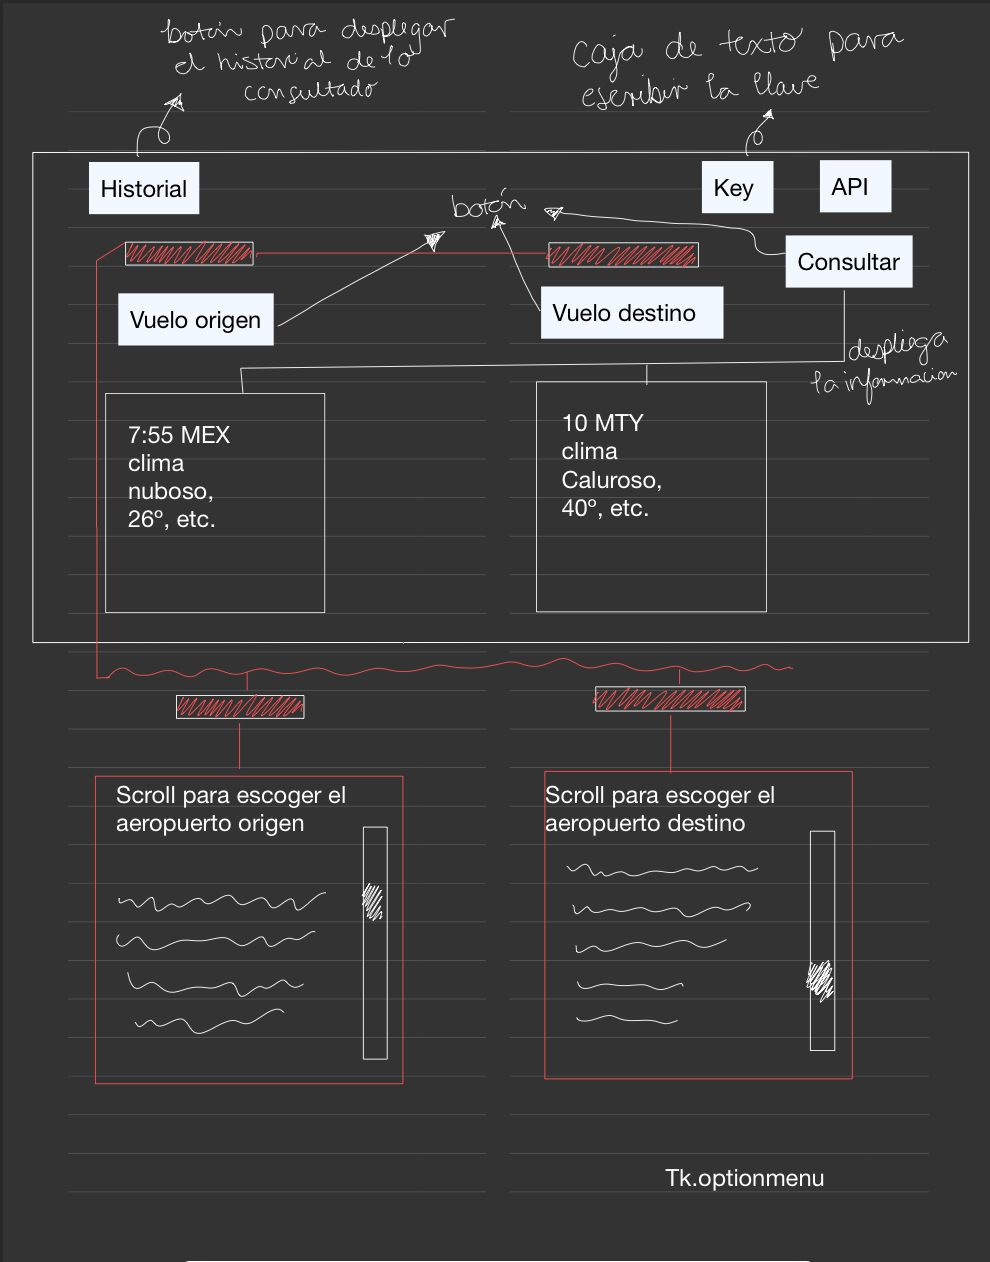
\includegraphics[scale=0.3]{figures/boceto}
  \caption{\label{fig:label} }
\end{figure}
\newpage
\section{Pseudocodigo}
\begin{algorithmic}[1]
  \For{cada vuelo}
  \If{ciudad de origen no esta registrada}
  \State{registrala en la primera casilla vacia}
  \EndIf
  \If{ciudad de destino no esta registrada}
  \State{registrala en el arreglo de la ciudad de origen}
  \EndIf
  \EndFor
  \For{ciudad de Origen}{ciudades}
  \State{Escribir en cada json el arreglo de ciudad Origen}
  \EndFor
  \State{Leer ciudad Origen}
  \State{Mostrar todos los destinos posibles dada la ciudad de origen}
  \State{climaOrigen = obtenerClima(ciudadOrigen, api)}
  \State{Leer ciudad destino}
  \State{climaDestino = obtenerClima(ciudadOrigen, api)}
  \State{Mostrar Clima}
  \State{Registrar el vuelo en un archivo}

  \Function{obtenerClima}{ciudadOrigen, api}
  \If{clima ya fue registrado en cache}
  \If{Han pasado mas de 30 min desde la ultima request}
  \State{realiza una peticion y guarda en cache}
  \EndIf
  \Else
  \State{realiza la peticion}
  \State{Guarda en los datos en la primera posicion disponible}
  \EndIf
  \EndFunction
\end{algorithmic}
\section{Mantenimiento}
En cuanto a mantenimiento se refiere si se podria dar seria tener la base de datos actualizada, si cambia el sistema operato ivdescargar las librerias y lenguajes ademas de que conforme se vaya mejorando la parte de encapsulacion creo que el programa podria acortarse el tamaño del programa.
\section{Pruebas}
Las pruebas las realizamos ingresando los datos manualmente y desde terminal para poder manipular mejor los datos, ya que como la interfaz es amigable con el usuario, son pocos los datos que el mismo manipula. Identificamos los datos como 
\subsection{Prueba con el archivo csv}
¿Que sucede si ingresamos el archivo csv incorrecto, es decir, nosotros requerimos que el archivo csv venga de la siguiente manera: $x,y,lat_o,lon_o,lat_d, long_d$, donde:
\begin{itemize}
\item $x$: nombre codigo de la ciudad de origen
\item $y$: nombre codigo de la ciudad de destino
\item $lat_o$: latitud de la ciudad de origen
\item $long_o$: longitud de la ciudad de origen
\item $lat_d$: latitud de la ciudad de destino
\item $long_d$: longitud de la ciudad de destino
\end{itemize}
por cada fila.

Si ingresamos un csv incorrecto nos mandara un mensaje diciendo que el archivo CSV es incorrecto y terminara la ejecucion del programa:\\
\begin{figure}[ht]
  \centering
  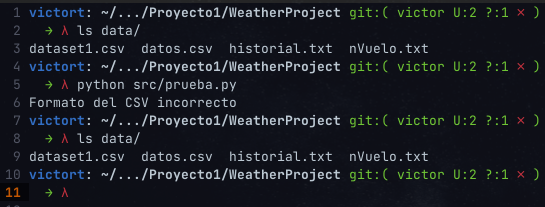
\includegraphics[scale=0.5]{figures/csvmalo}
  \caption{Ingresando un archivo csv incorrecto}
\end{figure}
\newpage
Ingresando un CSV bajo el formato correcto, ademas del programa ejecutarse con normalidad, observamos que en la carpeta data se crea unos archivos json por cada ciudad de origen:
\begin{figure}[ht]
  \centering
  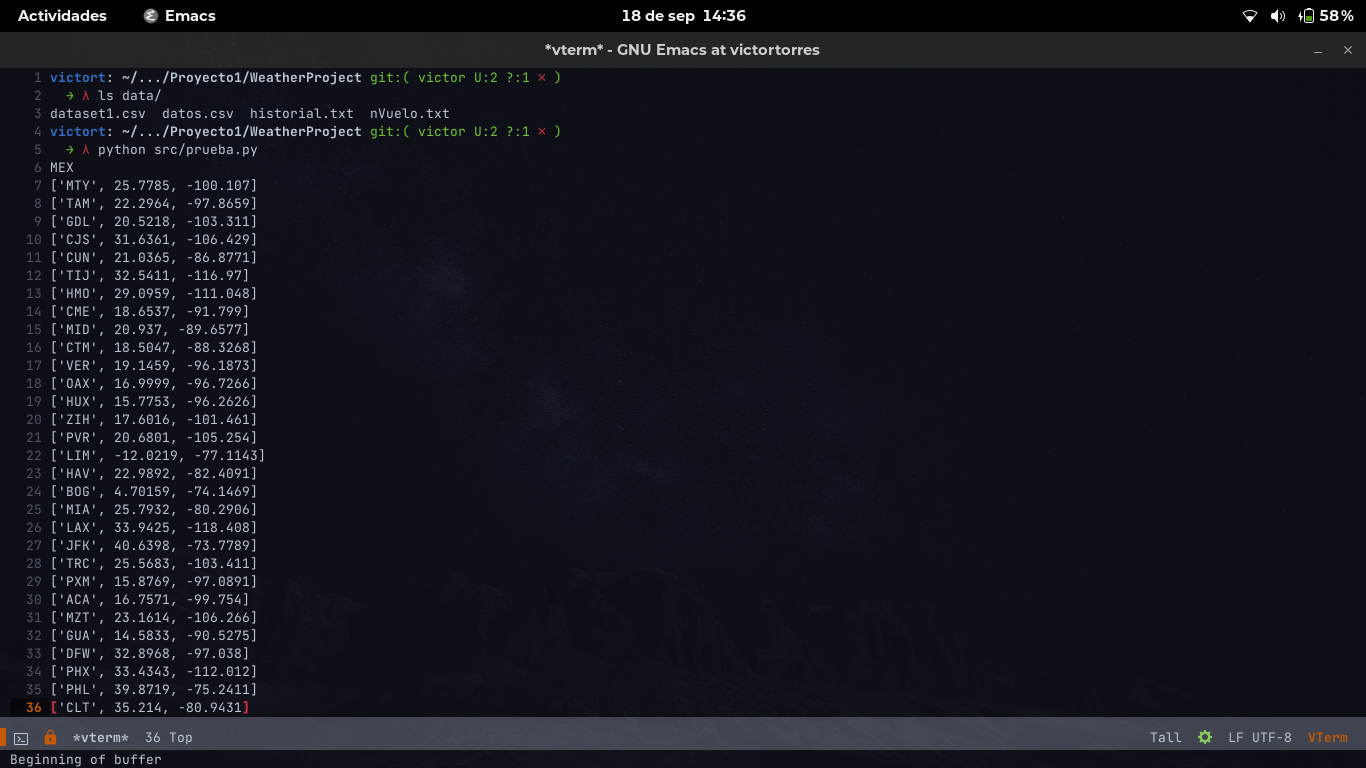
\includegraphics[scale=0.2]{figures/csv1}
  \caption{Ingresando un archivo csv con formato correcto}
\end{figure}

\begin{figure}[ht]
  \centering
  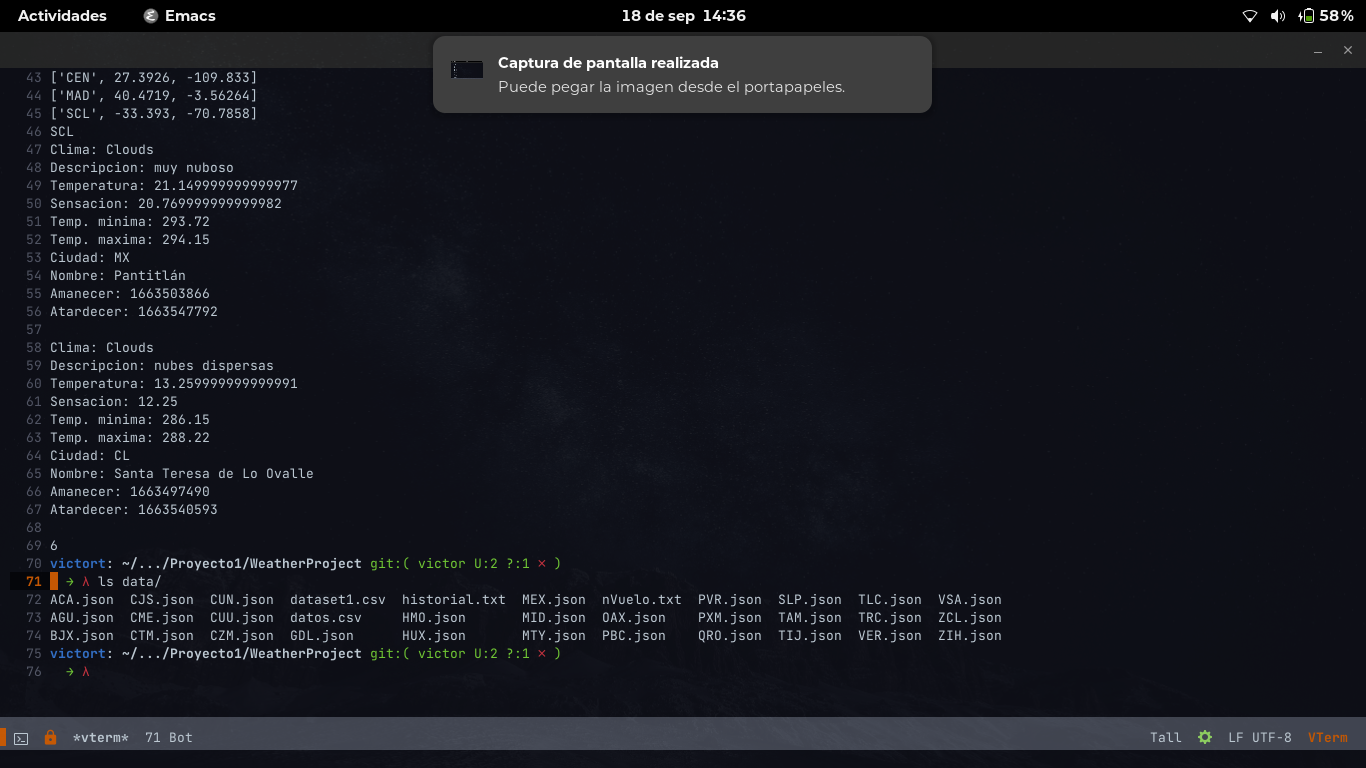
\includegraphics[scale=0.2]{figures/csv2}
  \caption{Ingresando un archivo csv con formato correcto}
\end{figure}
\newpage
\subsection{Prueba una ciudad inexistente}
¿Que pasa si ingresamos un nombre codigo de ciudad tanto de origen como de destino que no existe?

Si ingresamos un codigo (nombre acortado de la ciudad) de ciudad como ciudad de origen que no existe, el programa termina diciendo que la ciudad no existe
\begin{figure}[h!]
  \centering
  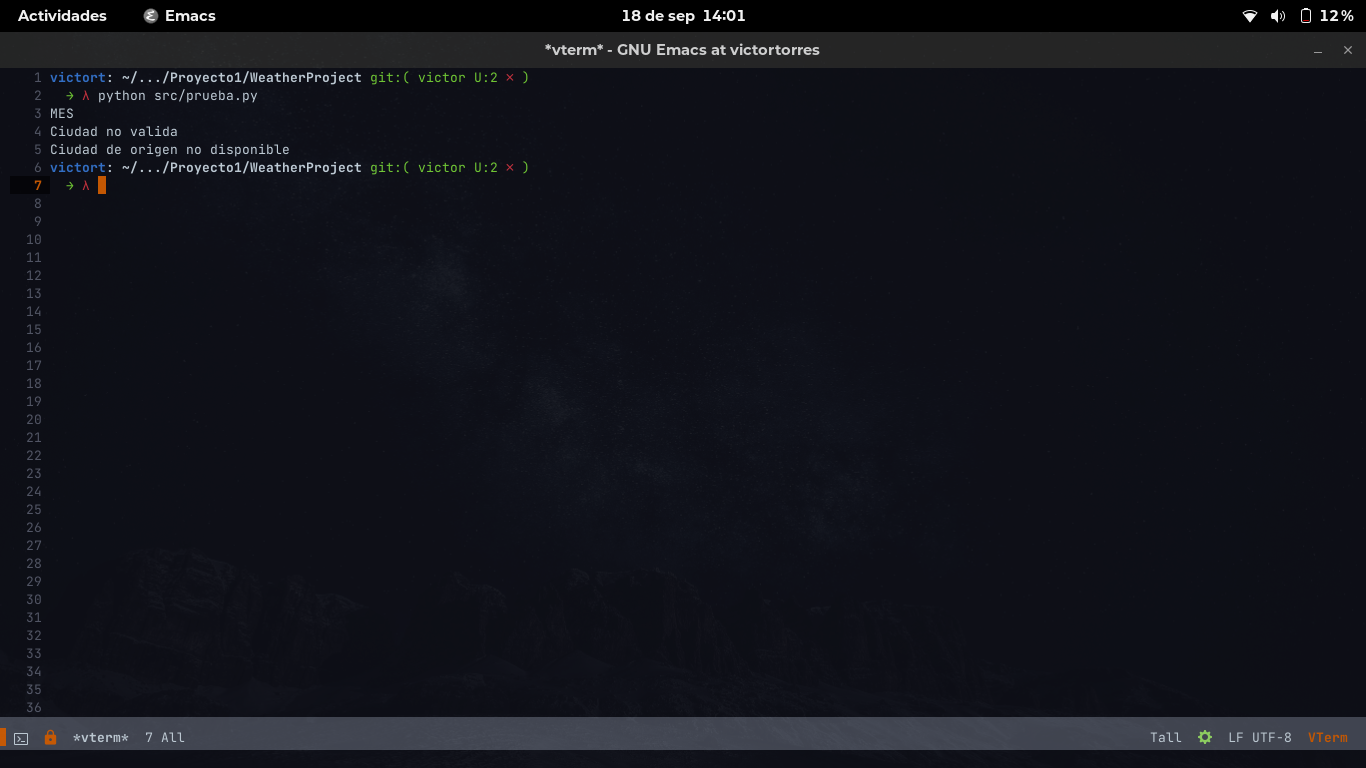
\includegraphics[scale=0.5]{figures/ciudadOmal}
  \caption{Ingresando una ciudad de origen inexistente}
\end{figure}

Si ingresamos un codigo de ciudad como ciudad de destino que no esta listada como destino disponible, el programa termina diciendo que esa ciudad de destino no existe.
\begin{figure}[ht]
  \centering
  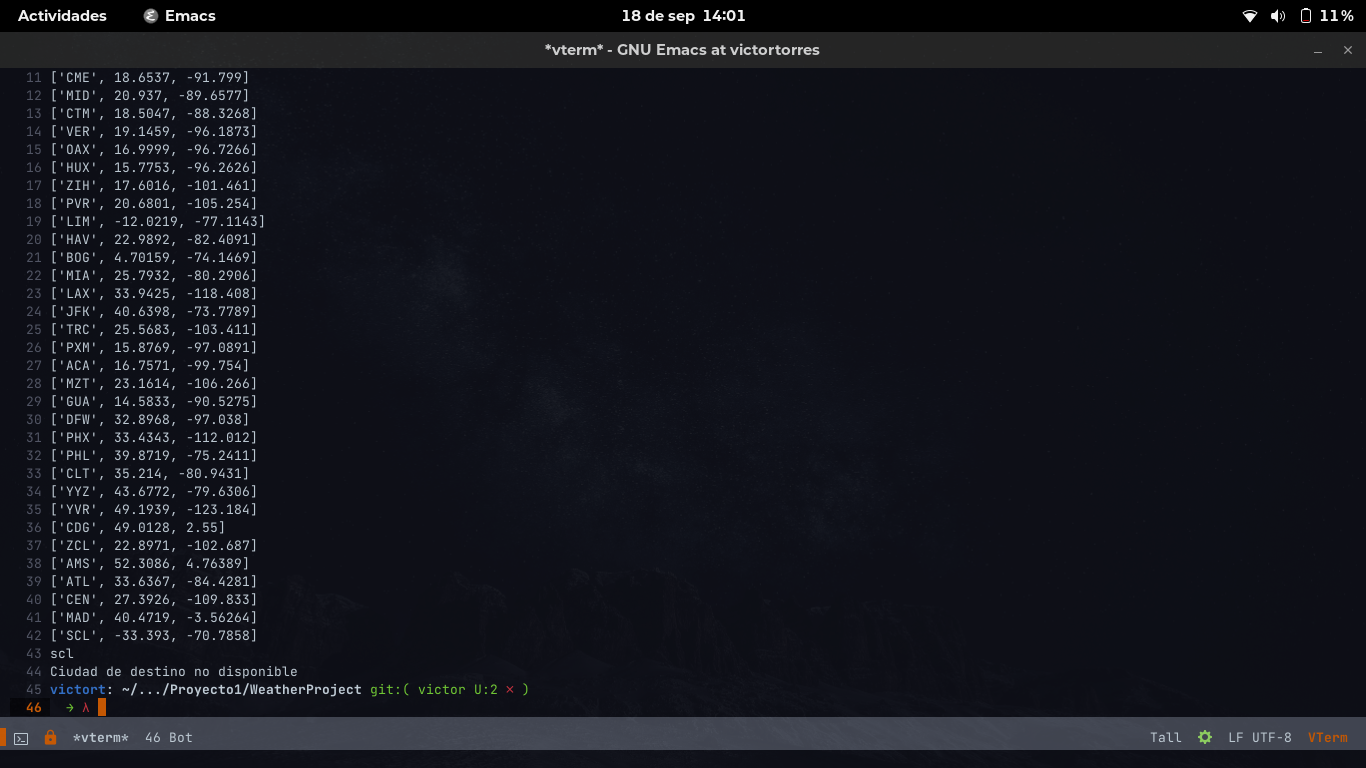
\includegraphics[scale=0.5]{figures/ciudadDmal}
  \caption{Ingresando una ciudad de destino inexistente}
\end{figure}
\newpage
Para ambos casos una prueba con entrada exitosa se ve asi:
\begin{figure}[ht]
  \centering
  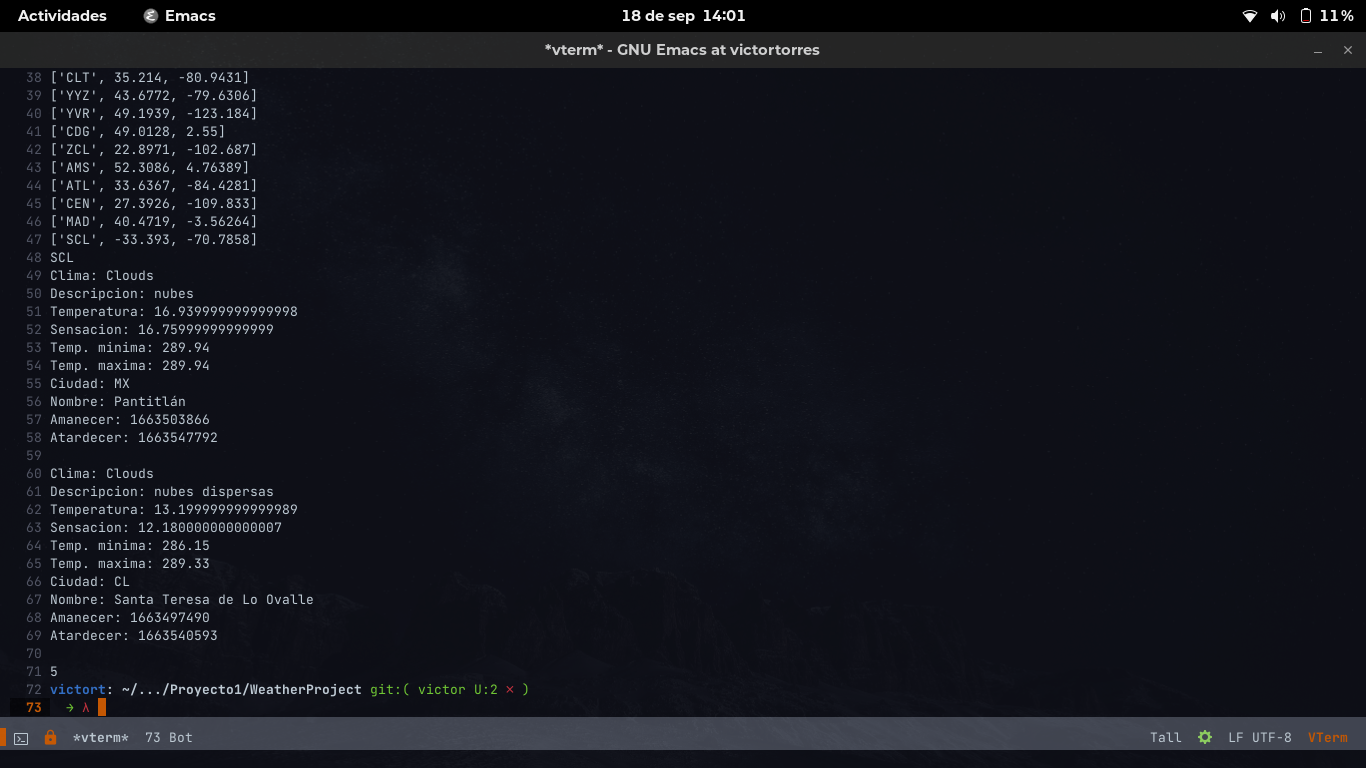
\includegraphics[scale=0.3]{figures/pruebaBuena}
  \caption{Prueba exitosa}
\end{figure}
\subsection{Una API erronea}
¿Que pasa si ingresamos una llave API no valida para la peticion de los datos?

Si corremos el programa con una llave API erronea, el programa lanzara un mensaje el cual dice que la peticion esta no autorizada
\begin{figure}[ht]
  \centering
  \includegraphics[scale=0.5]{figures/apimal}
  \caption{Haciendo una peticion con una llave API no valida}
\end{figure}
\newpage
Si ingresamos una llave API valida:
\begin{figure}[ht]
  \centering
  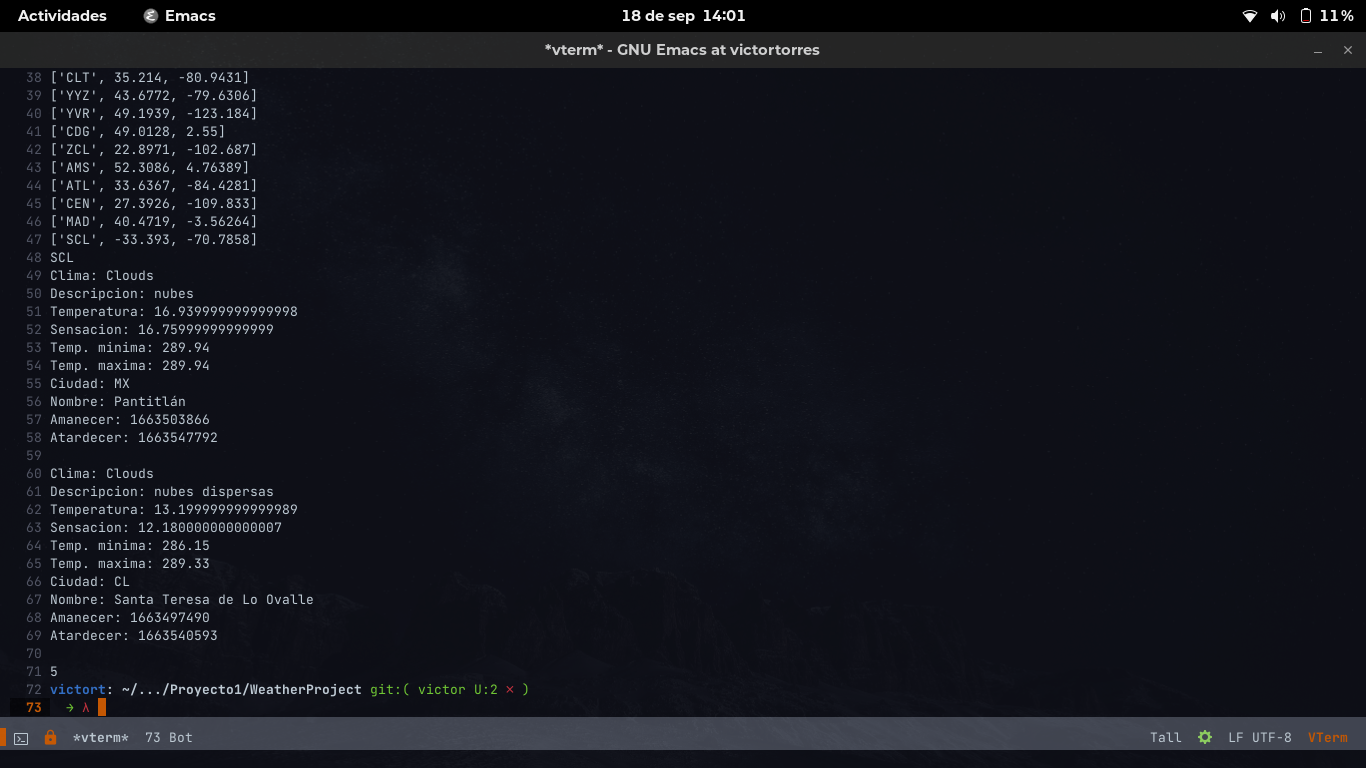
\includegraphics[scale=0.3]{figures/pruebaBuena}
  \caption{Llave API valida}
\end{figure}

\section{Costos}
El costo de desarrollo por la beta seria de \$1000, el de desarrollo final seria un costo total ya de \$2000 y por darle mantenimiento habria un costo de \$500


\end{document}
%%% Local Variables:
%%% mode: latex
%%% TeX-master: t
%%% End:
